DANA

%\subsection{Les ganglions de la base}
%%% Les ganglions de la base sont, comme leur nom l'indique, formés d'un ensemble de structures nerveuses enfouies profondément sous le cortex.%%%

%Plusieurs études ont été consacrées à la structure et à la physiologie des ganglions de la base \cite{Houk,Davis and Beiser 1995, Graybiel:1998, DeLong:2000}
%Les ganglions de la base peuvent être présentés comme deux structures d'entrée, deux structures de sortie et deux structures intrinsèques intermédiaires.
%Les structures d'entrées sont le striatum qui reçoit des signaux excitateurs de presque toutes les aires du cortex cérébral (sauf les aires primaires visuelle et auditive) 
%\cite{Cherubini:1988,Kemp:1970,kitai:1976,McGeer:1977} et le noyau sous-thalamique qui reçoit principalement des aires motrices du lobe frontal \cite{Fujimoto:1993, Monakow:1978, Rouzaire:1987}.
 
%\begin{figure}[htb]
%  \begin{center}
%    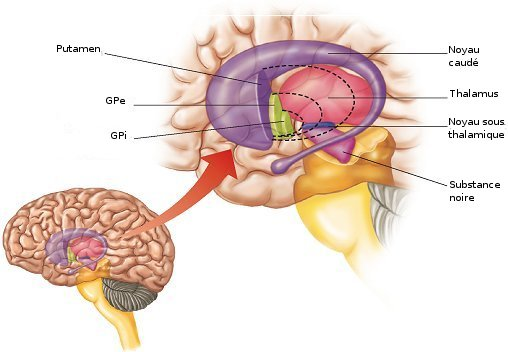
\includegraphics[width=0.6\textwidth]{Pics/BG1}
%  \end{center}
%  \caption {Les différents noyaux des ganglions de la base. Le striatum (STR) composé du noyau caudé et du putamen. Le pallidum composé du segment interne (GPi) et segment externe (GPE). La substance noire composée de la partie compacte (SNc) et la partie réticulée (SNr). Le noyau sous thalamique (STN).}
%  \label{fig:BG1}
%\end{figure}

%\subsubsection{Le striatum}

%Le striatum (STR, \textit{striatum}) est le plus large des noyaux gris centraux (10000000 neurones chacun connecté à 10000 synapses corticales). Il est composé du noyau caudé, du putamen et d'une partie différenciée connue sous le terme "striatum ventral"\footnote{Le striatum ventral est particulièrement impliqué dans la régulation des comportements motivés comme les processus naturels liés à l’obtention d’une récompense ou les processus pathologiques de l’addiction. %(Ikemoto and Panksepp, 1996; Koob, 1992; Koob and Bloom, 1988; Robbins et al., 1989; Robledo and Koob, 1993; Robledo et al., 1992; Salamone, 1994} qui englobe le noyau accumbens septi (NAcc, \textit{accumbens septi nucleus}), les parties ventromédiales du noyau caudé et du putamen et les cellules striatales des tubercules olfactifs.

%STR reçoit en effet de multiples afférences excitatrices glutamatergiques qui proviennent globalement de toutes les aires du cortex cérébral sauf l'aire visuelle primaire (V1, \textit{primary visual area}) et l'aire auditive primaire(A1, \textit{primary auditory area}) \cite{Albin:1995, Gerfen:1990, Cherubini:1988, Kemp:1970}. Outre le cortex, il reçoit des projections excitatrices des structures sous-corticales: thalamus (TH, \textit{thalamus}), hippocampe et amygdale \cite{Lapper:1992, Sadikot:1992}. 

%Il est constitué principalement ($90-90\%$) de neurones GABAergiques\footnote{L'acide $\gamma$-aminobutyrique, abrégé en GABA, est le principal neurotransmetteur inhibiteur du système nerveux central chez les mammifères et les oiseaux.} épineux moyens ( MSN, \textit{medium spiny neurons}). Au repos, ces neurones ont peu d'activité spontanée. Ils sont maintenus dans un état de faible excitabilité et sont peu réactifs aux influx corticaux excitateurs \cite{Nisenbaum:1995}. En conséquence, une forte activité synchronisée des projections cortico-striatales est nécessaire pour que les neurones de projection du striatum dépassent le seuil d'activation \cite {Mahon:2001, Mahon:2003}.

%Ces neurones projettent d'une part sur le segment interne du pallidum (GPi, \textit{internal globus pallidus}) et la substance noire réticulée (SNr, \textit { Substantia nigra pars reticulata}). D'autre part, ils projettent sur le noyau sous-thalamique (STN, \textit{subthalamic nucleus}) à travers le segment externe du pallidum (GPe, \textit{} external globus pallidus). Les neurones qui projettent vers un noyau ou un autre sont morphologiquement indifférenciables et topographiquement mélangés \cite{Feger:1984, Gerfen:1988, Parent:1989}. Ils commencent à décharger avant que le mouvement ne commence. Ceci suggère que le striatum participe à la programmation du mouvement en devenir. \cite{Lidsky:1985} ont signalé une activité neuronale striatale qui semblait être liée uniquement à des mouvements ou des stimuli sensoriels qui se produisent dans un contexte particulier. En effet, STR participe à filtrer les informations corticales les plus pertinentes et transformer les signaux corticaux selon le contexte afin d'inhiber localement les noyaux de sorties des BG permettant ainsi d'enlever l'inhibition tonique des générateurs de patterns moteurs (GPM, \textit{motor pattern generator}) reliés aux mouvements désirés mais il est également impliqué dans l'apprentissage de compétences motrices, perceptives et cognitives\cite{Joel:1994, Suzuki:2001}. 
 

%\subsubsection{Le noyau sous-thalamique}

%Le noyau sous-thalamique est le seul noyau excitateur des BG, il re\c coit des projections inhibitrices du GPe et ses neurones glutaminergiques renvoient des projections excitatrices répandues\footnote{efférences divergentes: chaque axone de STN innerve de nombreux neurones de GPi} aux GPi et SNr \cite{Parent:1993} permettant ainsi d'inhiber les MPG des mouvements concurrents. Il reçoit principalement des afférences excitatrices des aires motrices du lobe frontal.

%\subsubsection{Le pallidum externe}

%%Le segment externe du pallidum est une structure intermédiaire qui reçoit des projections inhibitrices de STR et d'autres excitatrices de STN et renvoie des projections GABAergiques inhibitrices vers STR et GPi mais majoritairement vers STN \cite{Rouzaire:1980}. Il semble agir en opposition aux projections striatales \cite{Alexander:1990}.
 


%\subsubsection{Le pallidum interne et la substance noire réticulée}

%Ces deux noyaux composés de neurones similaires sont considérés comme une seule structure fonctionnelle de sortie \cite {Carpenter:1981}. Ils sont toniquement actifs, i.e déchargent au repos à des taux élevés en l'absence de l'entrée striatale leur imposant une pause ou de réduire leur cadence de décharge. Ces structures pallidaux fonctionnent en utilisant un principe de désinhibition. Ayant feu . Parce un effet inhibiteur sur leurs cibles, l'effet net de l'entrée du striatum au GPi/SNr est une réduction de l'inhibition tonique exercée par les cellules pallidiales sur leurs cibles (désinhibition) permettant donc une augmentation du taux de décharge dans les cibles (thalamus, colliculus supérieur...). Donc leur désinhibition permet en particulier d'activer les aires motrices via le thalamus par excitations glutamatergique des aires corticales frontales et d'initier ainsi les mouvements moteurs bloqués toniquement \cite{Nauta:1966}. 






